\documentclass[10pt,landscape]{article}
\usepackage{multicol}
\usepackage{calc}
\usepackage{ifthen}
\usepackage[landscape]{geometry}
\usepackage{graphicx}
\usepackage{amsmath, amssymb, amsthm}
\usepackage{latexsym, marvosym}
\usepackage{pifont}
\usepackage{lscape}
\usepackage{graphicx}
\usepackage{array}
\usepackage{booktabs}
\usepackage[bottom]{footmisc}
\usepackage{tikz}
\usetikzlibrary{shapes}
\usepackage{pdfpages}
\usepackage{wrapfig}
\usepackage{enumitem}
\setlist[description]{leftmargin=0pt}
\usepackage{xfrac}
\usepackage[pdftex,
            pdfauthor={William Chen},
            pdftitle={Probability Cheatsheet},
            pdfsubject={A cheatsheet pdf and reference guide originally made for Stat 110, Harvard's Introduction to Probability course. Formulas and equations for your statistics class.},
            pdfkeywords={probability} {statistics} {cheatsheet} {pdf} {cheat} {sheet} {formulas} {equations}
            ]{hyperref}
\usepackage[
            open,
            openlevel=2
            ]{bookmark}
\usepackage{relsize}
\usepackage{rotating}

 \newcommand\independent{\protect\mathpalette{\protect\independenT}{\perp}}
    \def\independenT#1#2{\mathrel{\setbox0\hbox{$#1#2$}%
    \copy0\kern-\wd0\mkern4mu\box0}} 
            
\newcommand{\noin}{\noindent}    
\newcommand{\logit}{\textrm{logit}} 
\newcommand{\var}{\textrm{Var}}
\newcommand{\cov}{\textrm{Cov}} 
\newcommand{\corr}{\textrm{Corr}} 
\newcommand{\N}{\mathcal{N}}
\newcommand{\Bern}{\textrm{Bern}}
\newcommand{\Bin}{\textrm{Bin}}
\newcommand{\Beta}{\textrm{Beta}}
\newcommand{\Gam}{\textrm{Gamma}}
\newcommand{\Expo}{\textrm{Expo}}
\newcommand{\Pois}{\textrm{Pois}}
\newcommand{\Unif}{\textrm{Unif}}
\newcommand{\Geom}{\textrm{Geom}}
\newcommand{\NBin}{\textrm{NBin}}
\newcommand{\Hypergeometric}{\textrm{HGeom}}
\newcommand{\HGeom}{\textrm{HGeom}}
\newcommand{\Mult}{\textrm{Mult}}

\geometry{top=.4in,left=.2in,right=.2in,bottom=.4in}

\pagestyle{empty}
\makeatletter
\renewcommand{\section}{\@startsection{section}{1}{0mm}%
                                {-1ex plus -.5ex minus -.2ex}%
                                {0.5ex plus .2ex}%x
                                {\normalfont\large\bfseries}}
\renewcommand{\subsection}{\@startsection{subsection}{2}{0mm}%
                                {-1explus -.5ex minus -.2ex}%
                                {0.5ex plus .2ex}%
                                {\normalfont\normalsize\bfseries}}
\renewcommand{\subsubsection}{\@startsection{subsubsection}{3}{0mm}%
                                {-1ex plus -.5ex minus -.2ex}%
                                {1ex plus .2ex}%
                                {\normalfont\small\bfseries}}
\makeatother

\setcounter{secnumdepth}{0}

\setlength{\parindent}{0pt}
\setlength{\parskip}{0pt plus 0.5ex}

% -----------------------------------------------------------------------

\usepackage{titlesec}

\titleformat{\section}
{\color{blue}\normalfont\large\bfseries}
{\color{blue}\thesection}{1em}{}
\titleformat{\subsection}
{\color{cyan}\normalfont\normalsize\bfseries}
{\color{cyan}\thesection}{1em}{}
% Comment out the above 5 lines for black and white

\begin{document}

\raggedright
\footnotesize
\begin{multicols*}{3}

% multicol parameters
% These lengths are set only within the two main columns
%\setlength{\columnseprule}{0.25pt}
\setlength{\premulticols}{1pt}
\setlength{\postmulticols}{1pt}
\setlength{\multicolsep}{1pt}
\setlength{\columnsep}{2pt}

%%%%%%%%%%%%%%%%%%%%%%%%%%%%%%%%%%%%
%%% TITLE
%%%%%%%%%%%%%%%%%%%%%%%%%%%%%%%%%%%%

\begin{center}
    {\color{blue} \Large{\textbf{Probability for ML Cheatsheet}}} \\
   % {\Large{\textbf{Probability Cheatsheet}}} \\
    % comment out line with \color{blue} and uncomment above line for b&w
\end{center}

%%%%%%%%%%%%%%%%%%%%%%%%%%%%%%%%%%%%
%%% ATTRIBUTIONS
%%%%%%%%%%%%%%%%%%%%%%%%%%%%%%%%%%%%

\scriptsize

Compiled by Tu Nguyen Ngoc. Material based on Kelvin Murphy's book (\texttt{\href{https://probml.github.io/pml-book/}{@probml}}). Please share comments, suggestions, and errors at \url{github.com/nguyentuss/Probability-for-Machine-Learning-Cheatsheet}.

\begin{center}
    Last Updated \today
\end{center}

% Cheatsheet format from
% http://www.stdout.org/$\sim$winston/latex/

%%%%%%%%%%%%%%%%%%%%%%%%%%%%%%%%%%%%
%%% BEGIN CHEATSHEET
%%%%%%%%%%%%%%%%%%%%%%%%%%%%%%%%%%%%

\section{Introduction}\smallskip \hrule height 2pt \smallskip

 \subsection{Supervised Learning} 
    The task $T$ is to learn a mapping $f$ from $x \in X$ to $y \in Y$. The $x$ are also called the $\bold{features}$. The output $y$ is called the $\bold{label}$. The experience $E$ is given in the form of a set of $N$ input-output pair $\mathcal{D} = \{(x_n,y_n)\}, n = 1 \xrightarrow{} N$ is called $\textbf{training set}$. ($N$ is called the $\textbf{sample size}$. The performance $P$ depends on the type of output we want to predict.
\subsection{Classification}
    In classification problem, the output space is a set of C labels called $\textbf{classes}$, $Y = \{1,2,...,C\}$. The problem predicting the class label given a input is called $\textbf{pattern recognition}$.
    The goal of supervised learning in classification problem is want to predict the label. A common way to measure the perform on this task is called $\textbf{misclassification rate}$.
    \begin{center}
        $\mathcal{L}(\boldsymbol{\theta}) \triangleq \frac{1}{N} \sum_{n=1}^{N} \mathbb{I}\left(y_n \neq f(x_n; \boldsymbol{\theta})\right)$
    \end{center}
    Where $\mathbb{I}(e)$ is indicator function, which return 1 if the conditional is true, return 0 otherwise.
    We can also use the notation $\textbf{loss function}$ $l(y,\hat{y})$.
    \begin{center}
        $\mathcal{L}(\boldsymbol{\theta}) \triangleq \frac{1}{N} \sum_{n=1}^{N} \ell\left(y_n,  f(x_n; \boldsymbol{\theta})\right)$
    \end{center}
\subsection{Regression}
    Similarly to the classification problem, but now the output in regression are a real-value $y \in \mathbb{R}$ instead the discrete value $y \in \{1,...,C\}$; this is known as $\textbf{regression}$.
    So we need to use a different loss function. For regression, the most common choice is to use quadratic loss, or $\ell_2$ loss (L2 normalization)
    \begin{center}
        $\ell_2(y,\hat{y}) = (y - \hat{y})^2$
    \end{center}
    This penalizes large residuals $y-\hat{y}$. The empirical risk when use quadratic risk is equal to the $\textbf{Mean squared error}$ or $\textbf{MSE}$.
    \begin{center}
        $MSE(\boldsymbol{\theta})=\frac{1}{N} \sum_{n=1}^{N}(y_n-f(x_n;\boldsymbol{\theta}))^2$
    \end{center}
    \begin{minipage}{\linewidth}
            \centering
            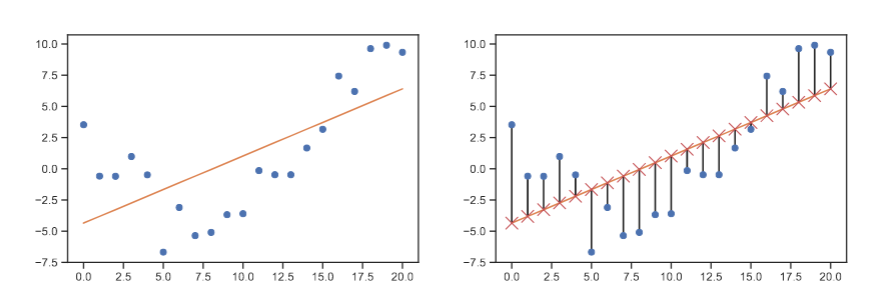
\includegraphics[width=3.5in]{figures/linear_regression.PNG}
    \end{minipage}
    An example of the regression model in 1d data, we can fix the data using the $\textbf{linear regression}$ model.
    \begin{center}
        $f(x;\boldsymbol{\theta})=b+wx$
    \end{center}
    Where w is the $\textbf{slope}$, b is the $\textbf{bias}$, and $\theta$ are the parameters of the model, we can minimize the sum square error.
    \begin{center}
        \[\hat{\boldsymbol{\theta}}=\arg\min_{\boldsymbol{\theta}}MSE(\boldsymbol{\theta})\]
    \end{center}
    If we have multiple input features, we can write
    \begin{center}
        $f(\mathbf{x};\boldsymbol{\theta})=b+w_1x_1+...+w_Dx_D=b+\mathbf{w^Tx}$
    \end{center}
    \begin{minipage}{\linewidth}
            \centering
            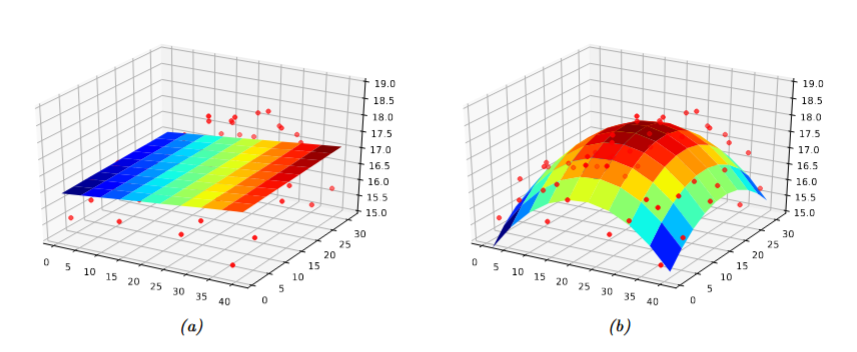
\includegraphics[width=3.5in]{figures/polynomial_regression.PNG}
    \end{minipage}
    We can improve the fit by using a $\textbf{Polynomial regression}$ model with degree $\mathcal{D}$. This now have the form 
    \begin{center}
        $f(x;\mathbf{w})=\mathbf{w^T}\phi(x)$
    \end{center}
    Where $\phi(x)$ are the feature vector derived from the input
    \begin{center}
        $\phi(x)=[1,x,x^2,...,x^D]$
    \end{center}

\subsection{Overfitting}
    Empirical risk (training loss function)
    \[
    \mathcal{L}(\boldsymbol{\theta}; \mathcal{D}_{\text{train}}) = 
    \frac{1}{|\mathcal{D}_{\text{train}}|} 
    \sum_{(\mathbf{x,y}) \in \mathcal{D}_{\text{train}}} 
    \ell(y, f(x; \boldsymbol{\theta}))
    \]

    The difference $\mathcal{L}(\boldsymbol{\theta};p^*)-\mathcal{L}(\boldsymbol{\theta};D_{train})$ called $\textbf{generalization gap}$.
    If a model has a large generalization gap (i.e., low empirical risk but high population risk), it is a sign that it is overfitting. In practice we don't know $p^*$. However, we can partition the data we do have into two subsets, known as the training set and the $\textbf{test set}$. Then we can approximate the population risk using the $\textbf{test risk}$:
    \[
    \mathcal{L}(\boldsymbol{\theta}; \mathcal{D}_{\text{test}}) = 
    \frac{1}{|\mathcal{D}_{\text{test}}|} 
    \sum_{(\mathbf{x,y}) \in \mathcal{D}_{\text{test}}} 
    \ell(y, f(x; \boldsymbol{\theta}))
    \]

    \begin{minipage}{\linewidth}
            \centering
            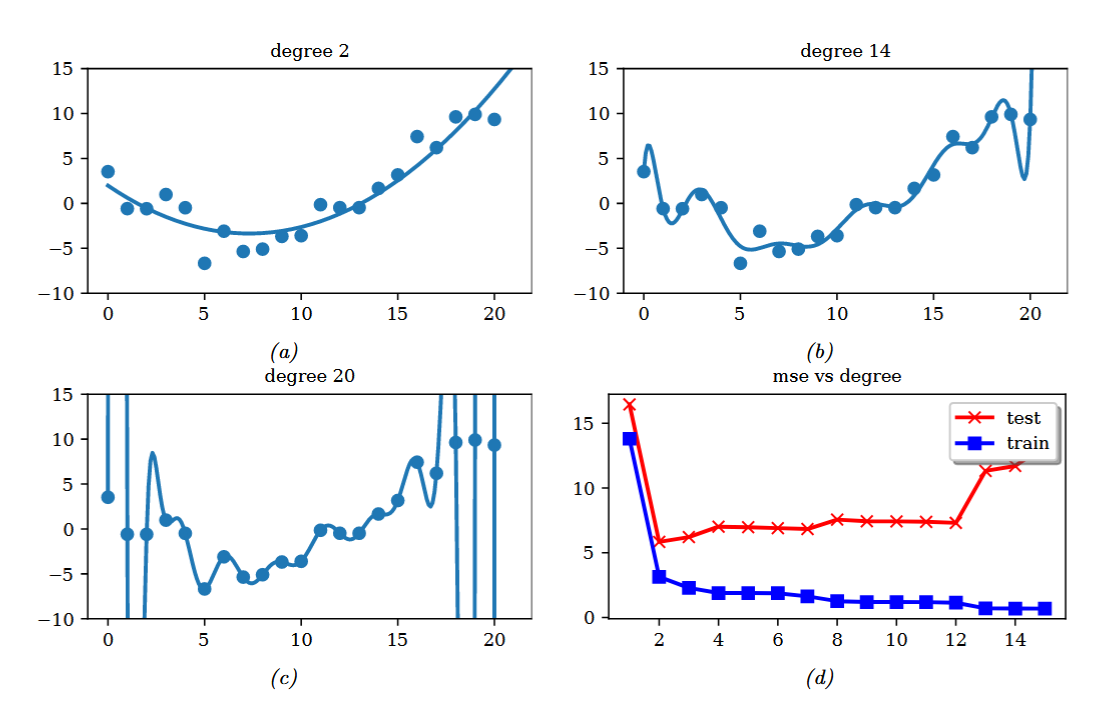
\includegraphics[width=3.5in]{figures/overfitting.PNG}
    \end{minipage}
    
    We can make the training loss function to zero if we increase the degree $\mathcal{D}$, but it will increase the testing loss function. The purpose about the prediction accuarcy on new data, A model that fit the training data but which is too much complex. It will call the $\textbf{overfitting}$. If $\mathbf{D}$ is too small, the model will be $\textbf{underfitting}$.
    
\subsection{Unsupervised learning}
    In supervised learning, we assume that each input $x$ in training set have a output targets $y$, and our goal is to learn the input-output mapping. Although this is useful, and difficult, supervised learning is just a to find a mathematical function to fit the data points. So go back to the unsupervised learning, we will opposed to just learning a mapping. We just get $\mathcal{D} = \{(x_n : n = 1 : N)\}$ without any ouputs $y_n$.This is called $\textbf{unsupervised learning}$.

    From a probabilistic perspective, we can view the task of unsupervised learning as fitting an unconditional model of the form $p(x)$, which can generate new data x, whereas supervised learning involves fitting a conditional model, $p(y|x)$, which specifies (a distribution over) outputs given inputs.

    Unsupervised learning avoids the needs of collect large labeled datasets for training, which can be often time comsuming and expensive and does not rely on manually labeled data or predefined categories, unlike supervised learning, which learns from labeled examples. Instead, unsupervised learning finds patterns, structures, or groupings in the data based on inherent similarities or relationships.
\subsection{Clustering}
    \begin{minipage}{\linewidth}
            \centering
            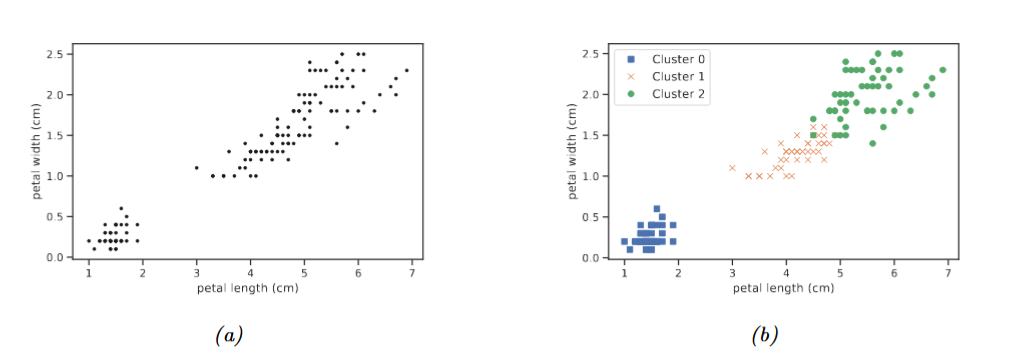
\includegraphics[width=3.5in]{figures/clustering.PNG}
    \end{minipage}
    A simple example of unsupervised learning is the problem of finding clusters in data. The goal is to partition the input into regions that contain “similar” points.
\subsection{Self-supervised learning}
    $\textbf{Self-supervised learning}$ that automatically generating $\textbf{labels}$ from $\textbf{unlabeled data}$. Try to learn to predict a color image from a grayscale image, or to mask out words in a sentence and then try to predict them given the surrounding context. The hope is that the resulting predictor $\hat{x}_1 = f(x_2;\boldsymbol{\theta})$. Where $x_2$ is the observed input and $\hat{x}_1$ is the predict output, will learn useful features from the data, that can be used in standard.
\subsection{Reinforcement learning}
    The system or agent has to learn how to interact with its environment. For example, creating a bot playing Mario, a bot will interact and integration with the world, run left or right or the bot will jump if they see a block stone.(\texttt{\href{https://pytorch.org/tutorials/intermediate/mario_rl_tutorial.html}{Click to see the detail}})
    \begin{minipage}{\linewidth}
            \centering
            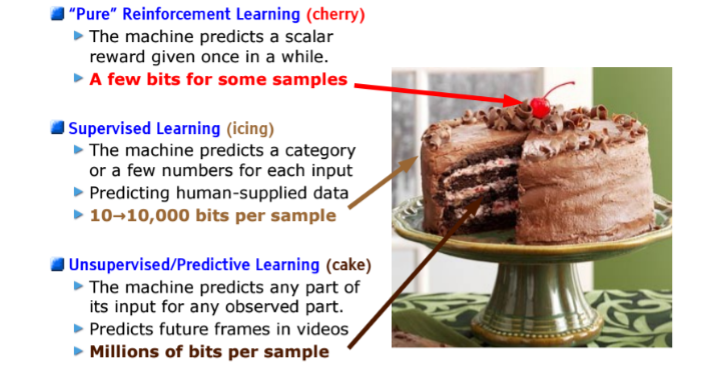
\includegraphics[width=3in]{figures/3typeML.PNG}
    \end{minipage}
\newpage
    
\subsection{Preprocessing discrete input data}


\end{multicols*}

\end{document}